\documentclass[letterpaper, 9pt]{article}
\usepackage[spanish]{babel}
\usepackage{authblk}
\usepackage[letterpaper, top=3cm, bottom=3cm, left=3cm, right=3cm, marginparwidth=1.75cm]{geometry}
\setlength{\affilsep}{2em} 
\usepackage{graphicx,color,xcolor, natbib, amsmath}
\usepackage[colorlinks=true, allcolors=blue]{hyperref}

\renewcommand*{\Affilfont}{\small\it}  

\title{\textbf{Estrategias para la Regulación de Precios y Creación de un Comedor Subsidiado en la UTB}}

\author[a]{Mauro González Figueroa \textit{(T00067622)}}
\author[a]{Valentina Del Rio Jimenez \textit{(T00081360)}}
\author[a]{Jorge Rueda Salgado \textit{(T00068722)}}
\author[a]{Joseph Gutiérrez de Piñeres \textit{(T00078923)}}
\author[a]{Isaac Navarro \textit{(T00068237)}}
\author[a]{Juan Jimenez Guardo \textit{(T00068278)}}

\affil[a]{Universidad Tecnológica de Bolívar. Parque Industrial y Tecnológico Carlos Vélez Pombo Km 1 Vía Turbaco. Cartagena de Indias, 130010, Colombia}
\affil[+]{Profesor: Leinys Melgarejo Causado (\textit{melgarejol@utb.edu.co})}

\begin{document}
\maketitle

\section{Problematica}
Los elevados precios de los alimentos dentro del campus universitario 
afectan negativamente la economía de los estudiantes y su acceso a una alimentación adecuada. 

\section{Objetivos}

\subsection{Objetivo General}
Implementar un sistema integral de regulación de precios y un comedor subsidiado para mejorar el acceso alimentario de los estudiantes de la UTB\@{}. 

\subsection{Objetivos Especificos}
\begin{enumerate}
      \item Diagnosticar la situación actual del servicio alimentario en la universidad. 
      
      \item Proponer un modelo de comedor subsidiado que responda a las necesidades estudiantiles. 
      
      \item Establecer convenios con proveedores locales para reducir costos.
       
      \item Diseñar estrategias de control de calidad y transparencia en la gestión alimentaria. 
\end{enumerate}

\noindent \textbf{Empresa/Organizacion:} Universidad Tecnológica de Bolívar- Campus Lemaitre, Cartagena 

\bigskip
\noindent \textbf{Productos:} Sistema de regulación de precios, comedor subsidiado, base de datos de proveedores, encuestas de satisfacción. 

\bigskip
\noindent \textbf{Localización:} Cartagena de Indias, Bolívar \textendash{} Campus UTB sede Lemaitre.

\bigskip
\noindent \textbf{Duración:} 20 Meses

\bigskip
\noindent \textbf{Costo del Proyecto:} \(\$92.900.000\)

\section{Impacto Social}
El proyecto no solo beneficiará a los estudiantes, sino que también:
\begin{itemize}
    \item Fomentará la economía local mediante alianzas con pequeños productores y proveedores.
    \item Reducirá la desigualdad alimentaria dentro del campus.
    \item Promoverá una cultura de sostenibilidad y responsabilidad social en la universidad.
\end{itemize}

\section{Resultados}

\section{Metodología}

\subsection{Diagnostico}

\begin{figure*}[ht]
     \centering
     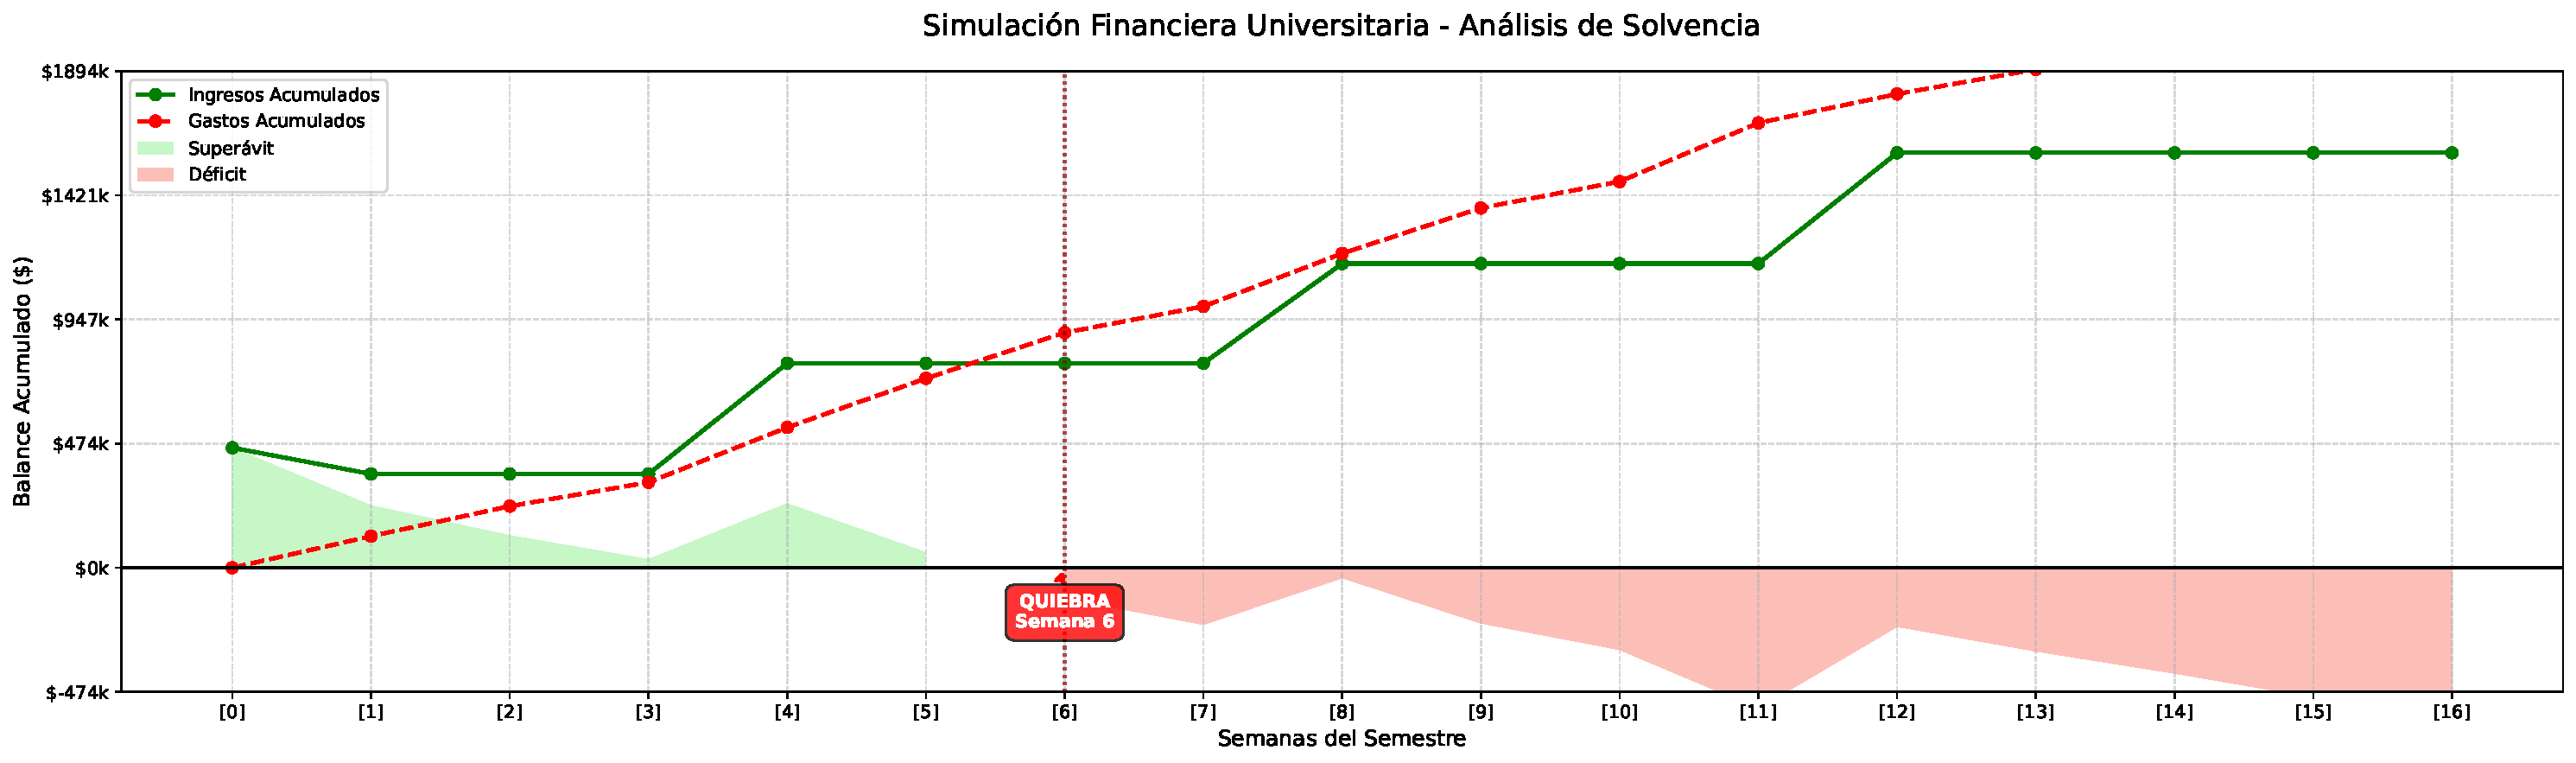
\includegraphics[width=\textwidth]{Images/graph.pdf} 
 
      \caption{Gráfico de líneas que ilustra la evolución de las finanzas de un estudiante a lo largo de un semestre académico. En este escenario, el estudiante cuenta con ingresos mensuales de \(\$400.000\) y un ahorro inicial de \(\$100.000\). El gráfico presenta dos componentes: las áreas en verde representan los ingresos acumulados a lo largo del tiempo, mientras que las áreas en rojo reflejan los gastos realizados. La línea vertical indica el punto crítico en el que los gastos igualan o superan los ingresos, conocido como ``semana de quiebre''. La simulación incorpora imprevistos y gastos adicionales ocasionales para reflejar un contexto realista (ver \url{https://github.com/MauroGonzalez51/college-prices-study} para mas informacion).}
\end{figure*}

\subsection{Diseño}

\bibliographystyle{unsrt}
\bibliography{./Bibliography/bibliography.bib}

\end{document}